 \newchapter{feedforward}{Feedforward Results}

This is the introductory text.

\newsection{gainScans}{Gain Scans}



\newsection{jitterRecord}{Lowest Achieved Phase Jitter}

The results presented in this section show the best downstream phase jitter currently achieved at CTF3 with the PFF correction. The dataset was taken on Friday 20th November 2015 at 15:38 as one of a sequence of short measurements fine-tuning the gain around the optimal value. Results from the other datasets in this sequence are discussed in the following section to demonstrate the phase stability achieved on longer time scales. The 15:38 dataset shown here comprises 150 pulses taken in interleaved mode, with the correction applied to the 75 odd indexed pulses and no correction applied to the remaining 75 even indexed pulses. The used gain in FONT5a units was 800, corresponding to a real applied correction of 1.13 times the upstream phase using the conversion factor calculated in Section \ref{ss:fontSetup}.

Naturally, this dataset was taken during the best beam conditions currently achieved at CTF3 in terms of phase propagation, taken just after a series of R56 and beam energy optimisations using the same methods discussed in Chapter \ref{c:phasePropagation}. In particular, the first attempt to smooth the upstream phase along the pulse by adjusting the waveform of the first klystron in the CTF3 injector (MKS02) as described in Section \ref{ss:t566Mitigation} yielded the highest upstream-downstream phase correlation achieved to date in normal conditions (higher correlations can be achieved by adding an additional jitter source upstream, as seen in Section \ref{s:pffNovelSetups}). 

Initially considering the mean pulse phase, the correlation with the PFF correction off in this dataset, as shown by the blue distribution of points in Figure \ref{f:BestFF_Real}, is \(0.93\pm0.04\). This gives a theoretical limit of a factor \(2.7\pm0.4\) reduction in the downstream jitter using Equation \ref{e:theoretJitOptGain}. The achieved uncorrected downstream mean phase jitter of \(0.74\pm0.06^\circ\) and downstream-upstream jitter ratio of \(1.1\pm0.1\) are also the lowest achieved at CTF3 to date. With this initial jitter and the theoretical reduction factor of \(2.7\pm0.4\) the lowest corrected downstream jitter that could be achieved is then \(0.27\pm0.05^\circ\). The aforementioned correlation and jitter ratio combine to give an optimal gain of \(1.0\pm0.1\) (Equation \ref{e:theoretOptGain}). With the actual gain used being 1.13 the PFF system would have been slightly over-correcting the downstream phase in these conditions, although the two values are almost consistent within the error bars and the achievable jitter degrades slowly about the optimal value so the effect should be negligible (Section \ref{ss:theoryJitter}) [TODO: Elaborate].

\begin{figure}
  \centering
  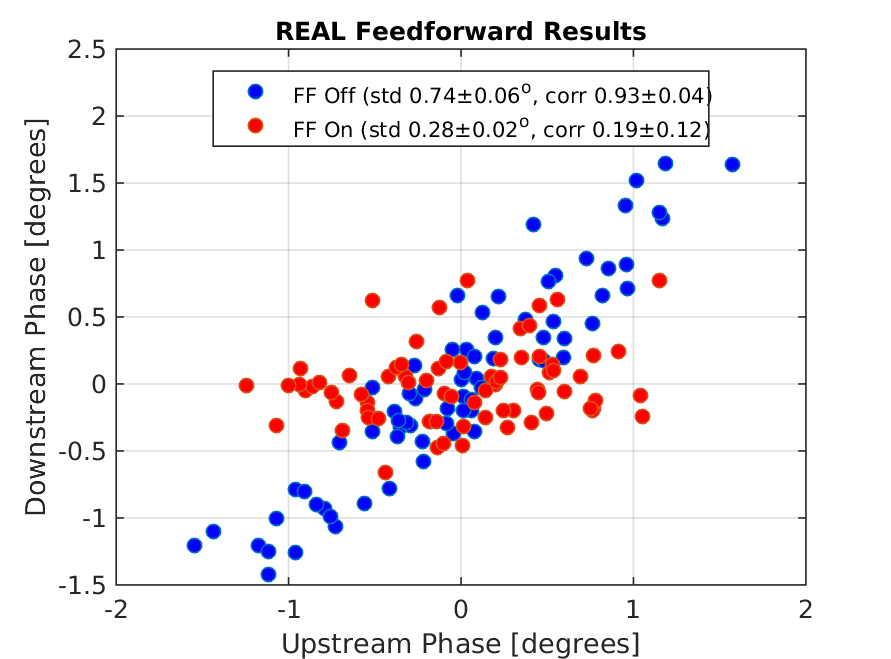
\includegraphics[width=0.75\textwidth]{Figures/feedforward/BestFF_Real}
  \caption{Mean phase.}
  \label{f:BestFF_Real}
\end{figure}

The red distribution of points in Figure \ref{f:BestFF_Real} then shows the effect of the PFF correction on the phase distribution. The correction acts to remove all correlation between the upstream and downstream phase, rotating the distribution as seen in the plot. The correlation is reduced from \(0.93\pm0.04\) to \(0.19\pm0.12\). As the used gain was slightly larger than optimal, a negative correlation might have been expected but this is not the case [TODO: why?]. The downstream phase jitter is reduced from \(0.74\pm0.06^\circ\) to \(0.28\pm0.02^\circ\), a reduction of a factor \(2.6\pm0.3\).  Within the error this agrees perfectly with the theoretical limit derived previously given the beam conditions in this dataset. It should be noted, however, that the measured upstream jitter of \(0.57\pm0.05^\circ\) across the pulses with the PFF correction on in this dataset is lower than the \(0.69\pm0.06^\circ\) measured with the PFF system off (Table \ref{t:BestFF}). This is simply a statistical effect rather than being a systematic difference between the odd and even pulses or an effect of the correction (which can only influence the downstream phase). Assuming the PFF on upstream jitter propagated downstream with the same ratio as the PFF off data, the true `natural' downstream jitter without the correction applied would have been \(0.61\pm0.09^\circ\) and the true factor reduction in the corrected jitter achieved with the PFF system would be decreased to \(2.2\pm0.4\). Assuming the upstream-downstream phase correlation was also not affected by this statistical fluctuation (so that the theoretical jitter reduction of a factor \(2.7\pm0.4\) still holds), a corrected jitter of \(0.23\pm0.05^\circ\) would have been theoretically possible for the PFF on pulses in this dataset. 

[TODO: Distribution of points at around 0.5 degrees downstream?]


With interleaved data it is also possible to simulate the expected effect of the correction empirically, as an additional point of comparison between the achieved and expected results plus as a verification of the theoretical predictions. The distribution of simulated corrected phases is shown in green on Figure \ref{f:BestFF_Simulated}. It is derived by taking the initial distribution with the PFF system off (blue points) and subtracting the upstream phase, multiplied by a gain factor, from the downstream phase. This exactly mimics what the feedforward system would have done if it had been applied to the even pulses in this dataset, and can be directly compared to the odd pulses taken at the same time with the real correction applied. In this example the simulation shown is the ideal case, considering a correction with infinite range and bandwidth applied with the optimal gain. As expected the simulated corrected downstream jitter of \(0.27\pm0.02\) agrees perfectly with the theoretical prediction of \(0.27\pm0.05^\circ\) previously derived. The achieved jitter of \(0.28\pm0.02\) matches both the theoretical and simulated jitter predictions within the error, giving confidence that the overall PFF setup in this dataset (after all the commissioning steps discussed in Chapter \ref{c:commissioning}) was close to optimal. There is perhaps some room for improvement due to the difference between the upstream jitter in the PFF on and off data, as mentioned previously, and this will be elaborated on in Section \ref{s:longPFF} below. Nevertheless, this result clearly demonstrates stability on the mean pulse phase approaching the CLIC target of 0.2 degrees at 12~GHz and demonstrates that achieving this stability with a PFF system is feasible.


\begin{figure}
  \centering
  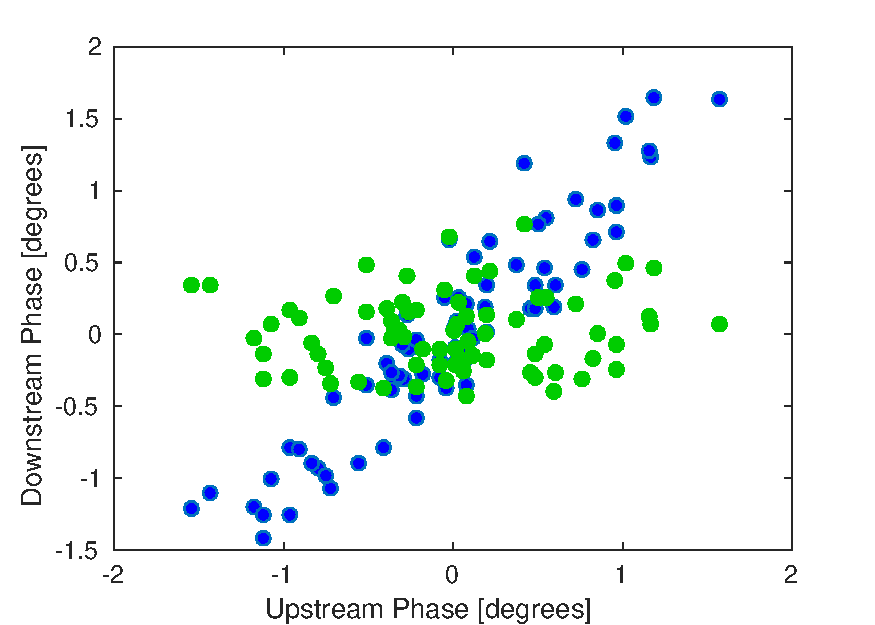
\includegraphics[width=0.75\textwidth]{Figures/feedforward/BestFF_Simulated}
  \caption{Simulated PFF.}
  \label{f:BestFF_Simulated}
\end{figure}


\begin{table}
  \begin{center}
    \begin{tabular}{| c | c | c | c |}
	   \hline
       Correction Status & Upstream Jitter & Downstream Jitter & Correlation \\ \hline
       FF Off & \(0.69\pm0.06^\circ\) & \(0.74\pm0.06^\circ\) & \(0.93\pm0.04\) \\
	   FF On & \(0.57\pm0.05^\circ\) & \(0.28\pm0.02^\circ\) & \(0.19\pm0.12\) \\
	   FF Simulated & \(0.69\pm0.06^\circ\) & \(0.27\pm0.02^\circ\) & \(0.06\pm0.12\) \\ \hline
    \end{tabular}
    \caption{Best PFF results.}
  	\label{t:BestFF}
  \end{center}
\end{table}

Moving on to the stabilisation of the phase along the pulse, Figure \ref{f:BestFF_MeanPhaseAlong} shows the mean phase along the pulse upstream, downstream with the PFF system off and downstream with the PFF system on. The vertical black lines mark the sample range that was used to calculate the mean phase results presented previously. The range is chosen to cover the maximal proportion of the pulse within which the the correction is not being saturated as a result of the phase sag (plus jitter) exceeding the \(\pm6^\circ\) correction range. It covers a total of 81 samples at 5.2 ns per sample, giving a total time span of 422~ns. The demonstration of \(0.28\pm0.01^\circ\) mean phase stability is therefore already on a much longer pulse than is needed for CLIC, where the combined pulse length is only 240~ns. [TODO: Any significant reduction in measured jitter by using 240ns window?] With the optimised phase propagation in place the overall shape of the upstream and (uncorrected) downstream phase, in green and blue respectively, along the pulse are very similar, although small uncorrelated variations are still visible. These uncorrelated differences are then visible in the corrected downstream phase (in red), although the overall ability of the PFF system to flatten the CTF phase sag within the sample range is strikingly clear. The original peak-to-peak variation in the mean downstream phase along the pulse of \(5.76\pm0.14^\circ\) with the correction off is reduced to \(0.65\pm0.07^\circ\) degrees with the correction applied.

Figure \ref{f:BestFF_Flatness} expresses the effect of the PFF system on the phase along the pulse in terms of the distribution of `flatness' values for each pulse in the data set with PFF system off and on. For each pulse, the flatness value is defined as the standard deviation of phase values across the sample range. In this case the flatness value of each pulse therefore corresponds to the standard deviation of 81 values (the length of the sample range). A pulse with a flatness value of zero would have constant phase across the whole sample range, with no small variations such as those seen in Figure \ref{f:BestFF_MeanPhaseAlong}. The value is also insensitive to the jitter on the overall mean pulse phase seen earlier in Figure \ref{f:BestFF_Real}. In Figure \ref{f:BestFF_Flatness}, the uncorrected downstream pulse flatness, dominated by the phase sag at CTF3, of \(1.68\pm0.02^\circ\) is reduced to \(0.26\pm0.01^\circ\) with the correction applied. On average, the corrected pulses are \(6.5\pm0.3\) times `flatter' than the uncorrected pulses.

Finally, Figure \ref{f:BestFF_StdPhaseAlong} shows the overall phase jitter at each sample along the pulse upstream and downstream with the PFF system off and on. These jitter values contain components coming from both the jitter on the overall mean pulse phase discussed initially and from the variations along the pulse (the non-zero flatness of each pulse). These jitter values are therefore larger and taking the mean sample jitter within the sample range an initial downstream jitter of \(0.72\pm^\circ\) is reduced to \(0.36\pm^\circ\) by the correction in this case, a factor 2 reduction. There are also variations of up to a factor 2 in the jitter that was achieved at each sample point, the lowest jitter being \(0.27\pm^\circ\) at time 797~ns on the x-axis and the worst \(0.52\pm^\circ\) at time 552~ns. [TODO: Error bars]

[TODO: Simulation of results along pulse]

\begin{figure}
  \centering
  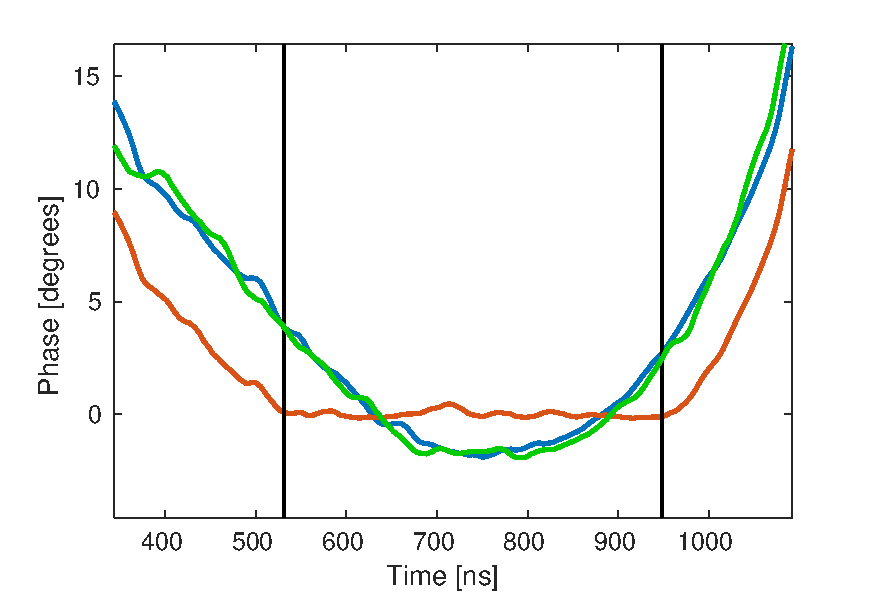
\includegraphics[width=0.75\textwidth]{Figures/feedforward/BestFF_MeanPhaseAlong}
  \caption{Mean phase along.}
  \label{f:BestFF_MeanPhaseAlong}
\end{figure}

\begin{figure}
  \centering
  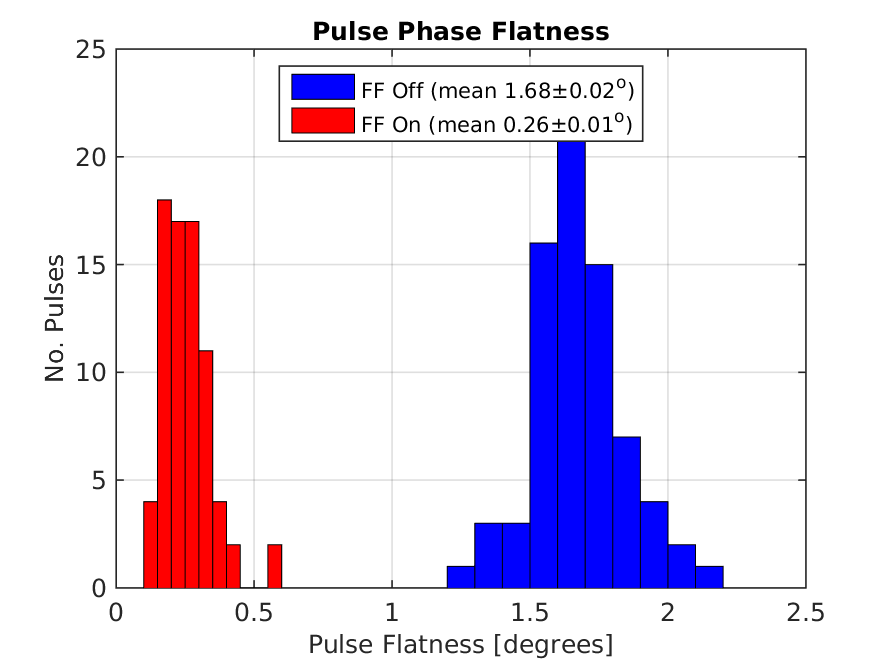
\includegraphics[width=0.75\textwidth]{Figures/feedforward/BestFF_Flatness}
  \caption{Flatness.}
  \label{f:BestFF_Flatness}
\end{figure}

\begin{figure}
  \centering
  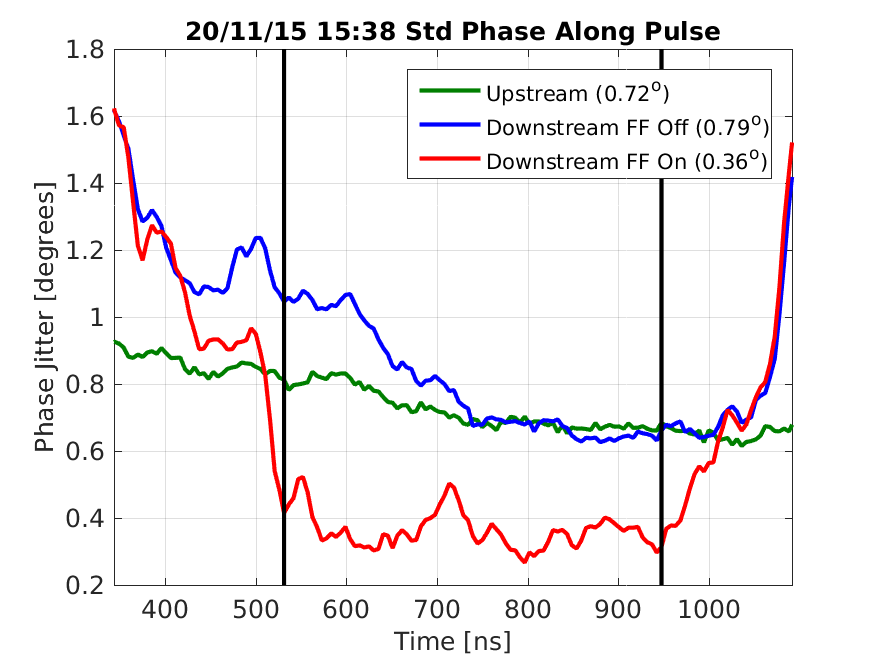
\includegraphics[width=0.75\textwidth]{Figures/feedforward/BestFF_StdPhaseAlong}
  \caption{Std phase along.}
  \label{f:BestFF_StdPhaseAlong}
\end{figure}

\newsection{longPFF}{Correction on Longer Time Scales}

At CLIC 0.2 degrees phase stability would clearly have to be maintained for much longer time scales than a few minutes. This section therefore discusses the status of the correction across longer time scales, using data from around 15:30 to 18:00 on the 20th November 2015, the same day as the record result previously shown which was taken during this period at 15:38. The PFF system was not operated continuously throughout this two and a half hour window but 15 individual datasets of a few hundred pulses each were taken and these results have been combined to create a large sample of 3083 interleaved pulses (1541 with the correction on and 1542 with the correction off).

\begin{landscape}

\begin{figure}
  \centering
  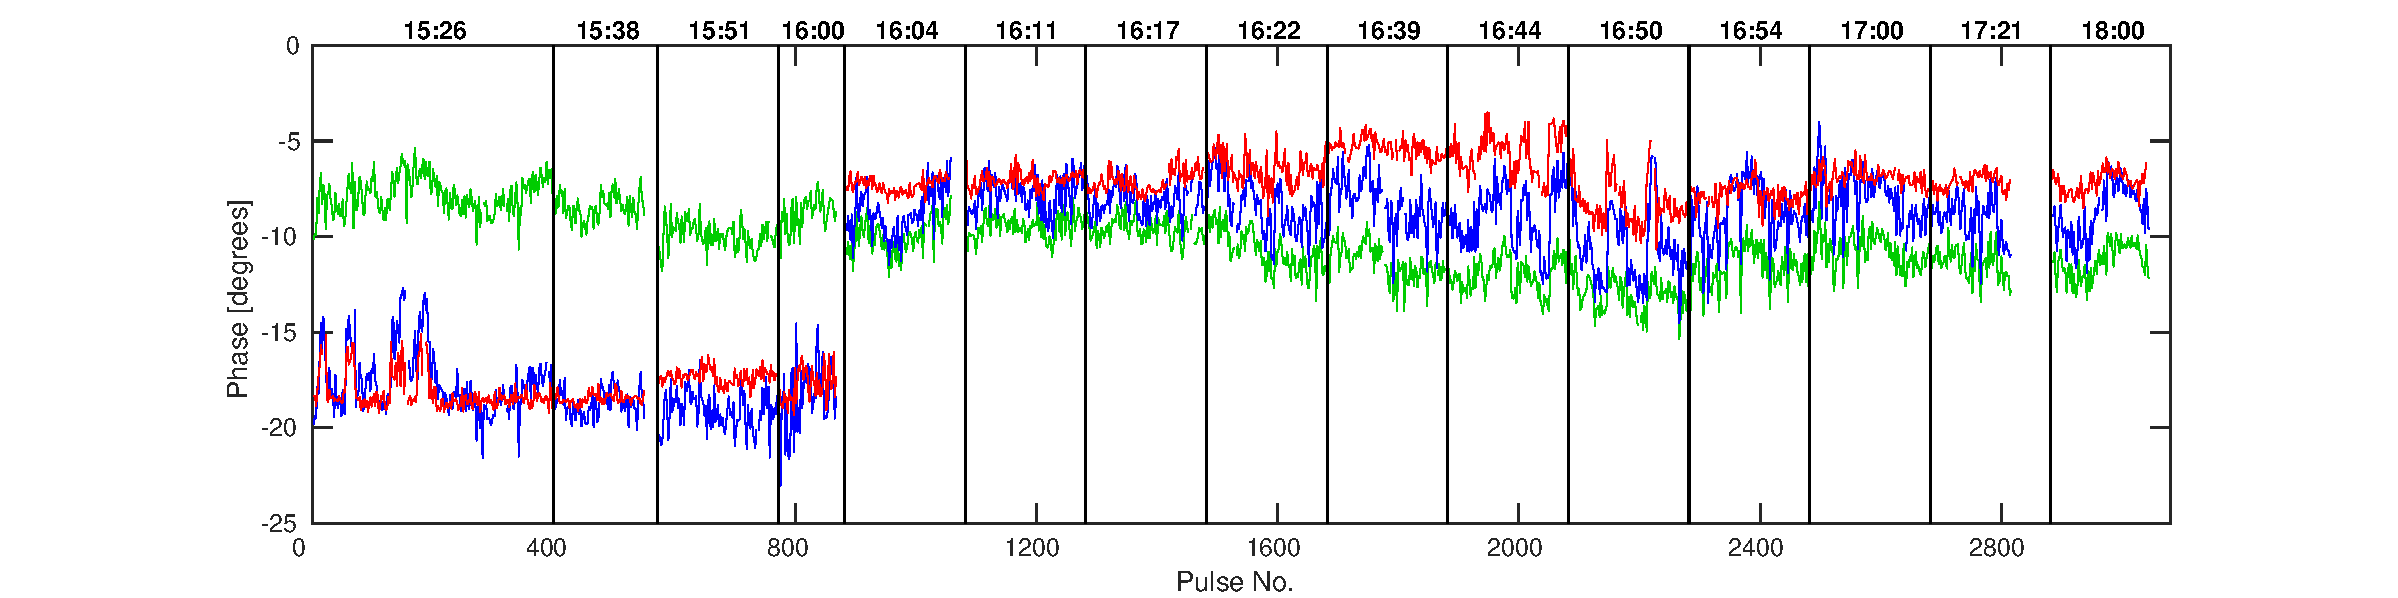
\includegraphics[width=\hsize]{Figures/feedforward/longFF_noMeanSubHistory}
  \caption{History of mean phase across datasets.}
  \label{f:longFF_noMeanSubHistory}
\end{figure}


\begin{figure}
  \centering
  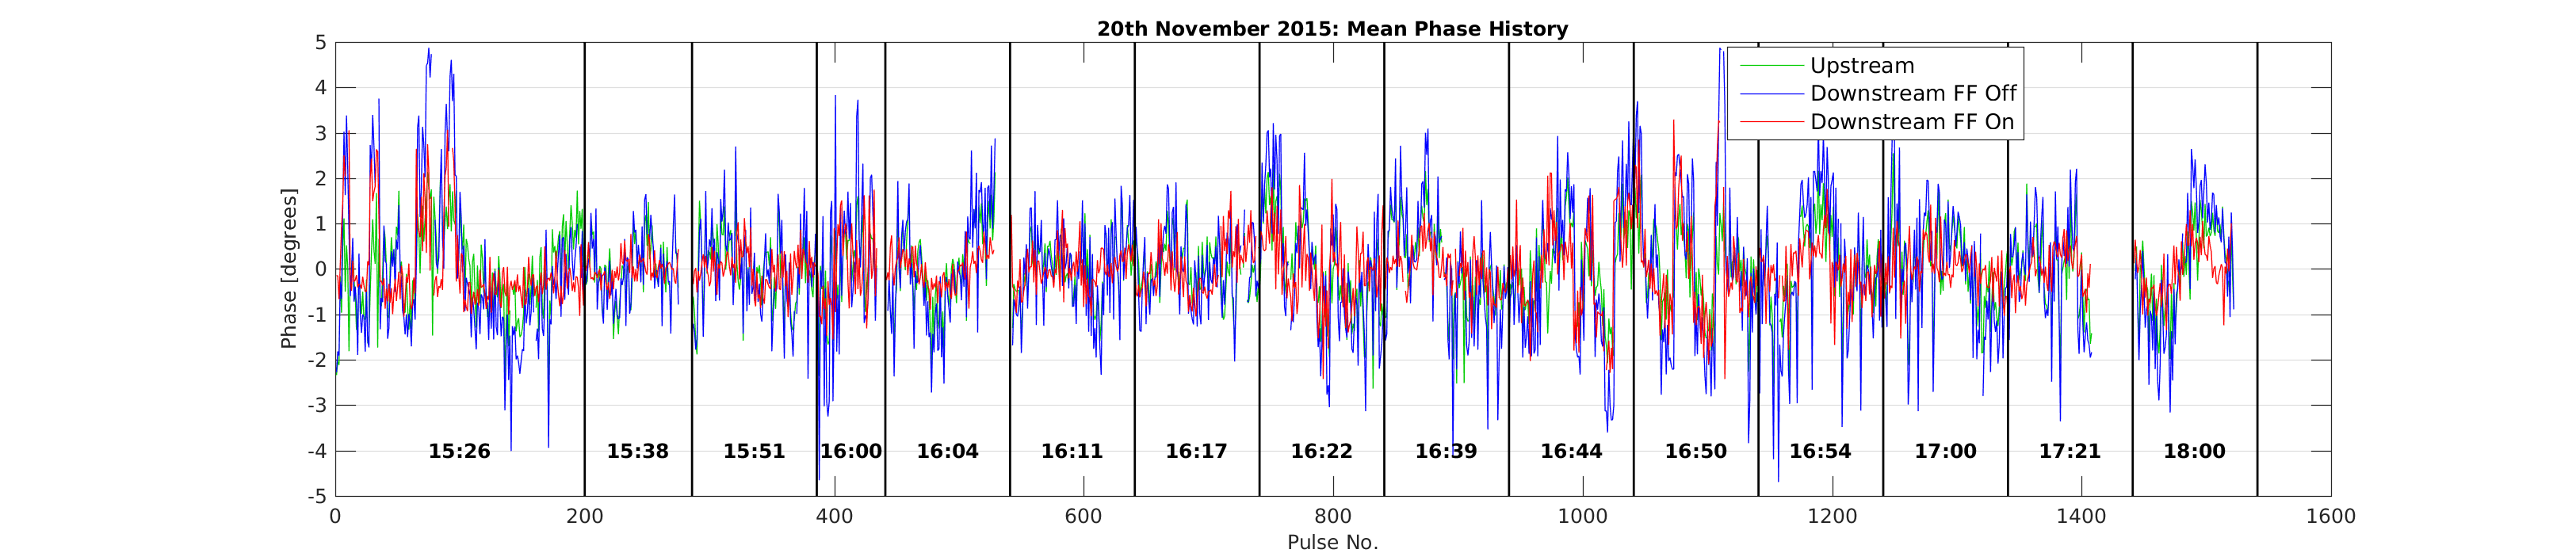
\includegraphics[width=\hsize]{Figures/feedforward/longFF_history}
  \caption{History of mean phase across datasets, with mean subtraction.}
  \label{f:longFF_history}
\end{figure}

\end{landscape}

The raw history of the mean phases upstream and downstream with the correction on and off in the combined data are shown in Figure \ref{f:longFF_noMeanSubHistory}. The time span of each individual dataset is marked by vertical black lines and the times displayed on the plot represent the start time of each dataset. 

Over the course of the afternoon the mean upstream phase, in green, varies by ten degrees peak-to-peak or \(1.75 \pm 0.02^\circ\) in terms of jitter. Small drifts of up to a few degrees in the upstream phase are not an issue for the performance of the PFF correction providing the correlation between the upstream and downstream phase is not degraded. In some cases upstream phase drifts may lead to a loss in correlation, this could be the case if the source of the drift is a variation in beam energy due to the issues discussed in Chapter \ref{c:phasePropagation}, for example. The variation of the correlation between datasets is discussed later in this section.

Larger changes in the upstream phase such as the ten degree fluctuation seen here will impact the PFF performance purely via the limited correction range of \(\pm6^\circ\) combined with the phase sag along the CTF pulse. Indeed the PFF prototype's main purpose is not to remove any large, slow phase drifts but rather the faster pulse-to-pulse jitter and high frequency variations along the pulse. The phase offset applied by the PFF correction at each sample along the downstream phase, \(\Delta\phi_d(t)\), is given by:

\begin{eqnarray}
	\Delta\phi_d(t) = \begin{cases}
	-6^\circ, &  \text{if $g\phi_u(t) \geq+6^\circ$.}\\
	+6^\circ, &  \text{if $g\phi_u(t)\leq-6^\circ$}.\\
	-g\phi_u(t), &  \text{otherwise.}
	\end{cases}
	\label{e:limCorrection}
\end{eqnarray}

Where \(\phi_u(t)\) is the upstream phase at each sample point and \(g\) is the gain factor used. As the optimal gain (Section\ref{ss:theoryGain}) for the correction is typically larger than one due to the slight amplification in the downstream phase jitter with respect to the upstream jitter the range of the PFF system in terms of the upstream phase is less than \(\pm6^\circ\) (for example \(\pm5.3^\circ\) for the 15:38 jitter record dataset with a gain of 1.13). Any point along the upstream phase with \(|g\phi_u(t)| > 6^\circ\) receives the maximum \(6^\circ\) phase shift downstream but can not corrected to zero, with this remaining residual degrading the corrected phase jitter that can be achieved. Samples with  \(|g\phi_u(t)| > 5^\circ\) will also receive a slightly non-optimal correction due to the effects of the amplifier entering saturation, shown in Section \ref{ss:kickLin}, although this is negligible and not considered in the discussion here [TODO: Calculate how significant]. 

Figure \ref{f:longFF_fractInRange} shows the fraction of pulses for which the optimal correction is within the correction range in the combined dataset. During the setup of the PFF system it is necessary to choose the zero point for the correction, i.e. the incoming upstream phase at which the correction output to the kickers is 0~V. This is done in the PFF firmware on the FONT5a board by varying a channel offset applied to the ADC to which the mixer signal from the upstream phase monitor is connected. In terms of equation \ref{e:limCorrection} this is equivalent to adding a constant offset to \(\phi_u\) across the full pulse length. If on the FONT5a board the offset has been set up perfectly, so that the mean voltage sent to the kickers across the afternoon is zero, the effects of limited correction range are small, as the full \(\pm6^\circ\) range can be used to remove phase jitter rather than any static phase offsets. In this case the ideal correction across a 310~ns portion of the pulse is within the \(\pm6^\circ\) range 96\% of the time.

\begin{figure}
  \centering
  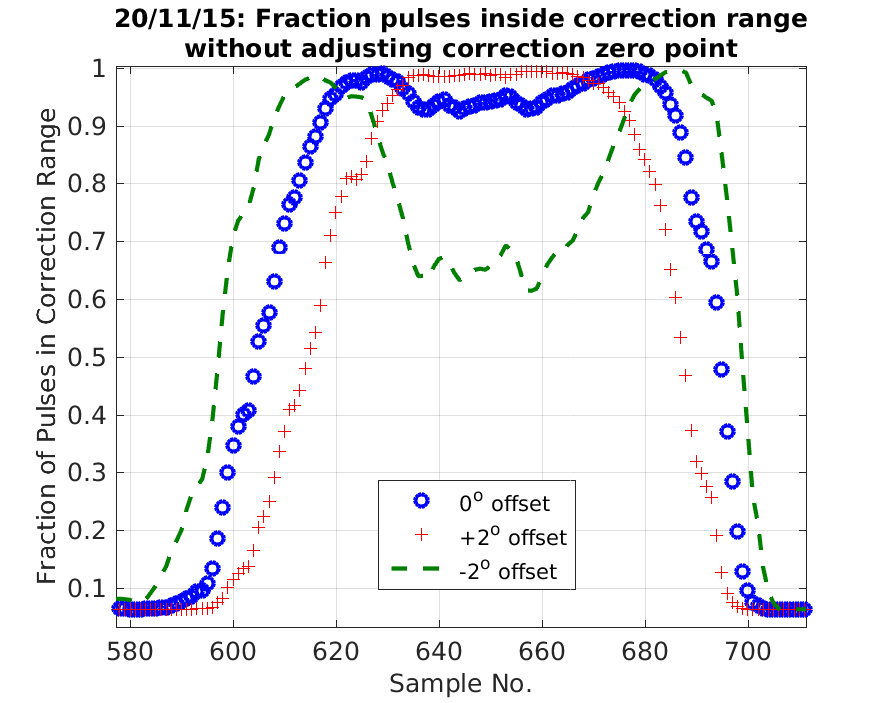
\includegraphics[width=0.45\textwidth]{Figures/feedforward/longFF_fractInRange}
  \caption{Fraction of pulses outside the correction range along the pulse.}
  \label{f:longFF_fractInRange}
\end{figure}

However, as to date this offset has been set up manually small deviations from the ideal case are possible. Figure \ref{f:longFF_fractInRange} also shows the fraction of pulses within the correction range if there is a static two degree offset in the upstream phase. In this case as many as 39\% of pulses are outside the correction range within the normally correctable central region of the pulse. To mitigate these effects and to get the largest reduction in jitter possible within each individual dataset the centring of the upstream phase in the correction range on the FONT5a board is normally adjusted between datasets. As a consequence of this differences in the upstream phase between datasets are not removed in the corrected downstream phase, as the zero point for the PFF correction is effectively moving with the phase drifts during the afternoon. These remaining slow drifts could be removed at CTF3 using a secondary ``slow phase feedback", also utilising the TL2 chicane, which is the focus of Section \ref{s:slowCorr}.

The accuracy to which the channel offset for the upstream phase has been selected can be inferred by comparing the mean downstream phase in each dataset with the correction on (red) and off (blue) in Figure \ref{f:longFF_noMeanSubHistory}. In the ideal case the mean phase should be identical with the PFF system on and off, so that the full correction range is being used to correct jitter about the mean as mentioned previously. Although this is the case for some datasets, such as the 15:38 dataset, a clear offset between the two is often present, most visible in the datasets between 16:39 and 16:50 in which the corrected phase is clearly shifted several degrees with respect to the uncorrected phase. The offset in each dataset is plotted in Figure \ref{f:longFF_phaseOffset} [TODO: Change to table?]. In the region between 16:39 and 16:50 the offset falls below \(-3^\circ\). The mean offset across the combined dataset is \(-1.4^\circ\) [TODO: Calc error, weight by datset lengths]. Even with the clearly non-optimal set point for the offset there should be almost no effect on the correction [TODO: calculate, plot].

\begin{figure}
  \centering
  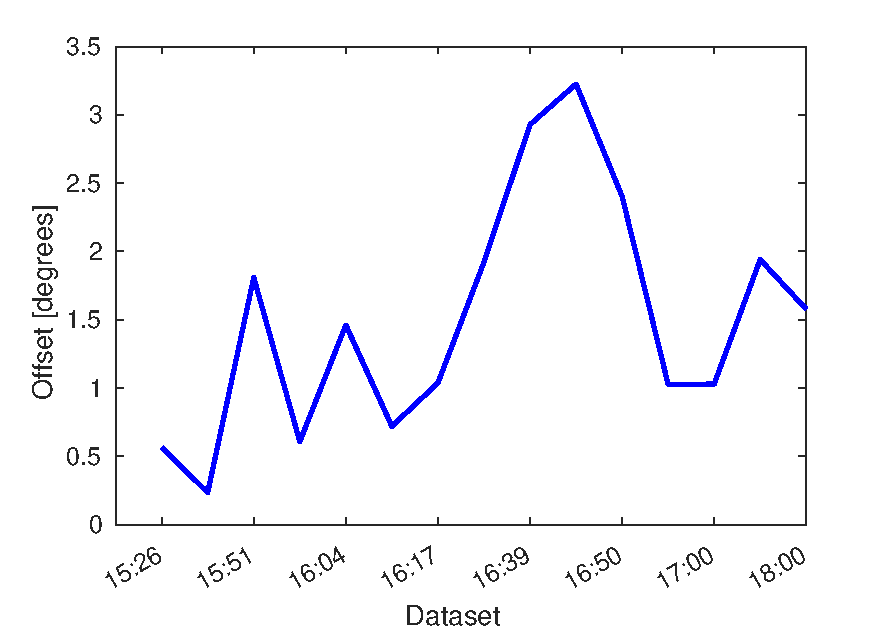
\includegraphics[width=0.45\textwidth]{Figures/feedforward/longFF_phaseOffset}
  \caption{Offset between downstream phase with FF off and FF on.}
  \label{f:longFF_phaseOffset}
\end{figure}



\begin{figure}
  \centering
  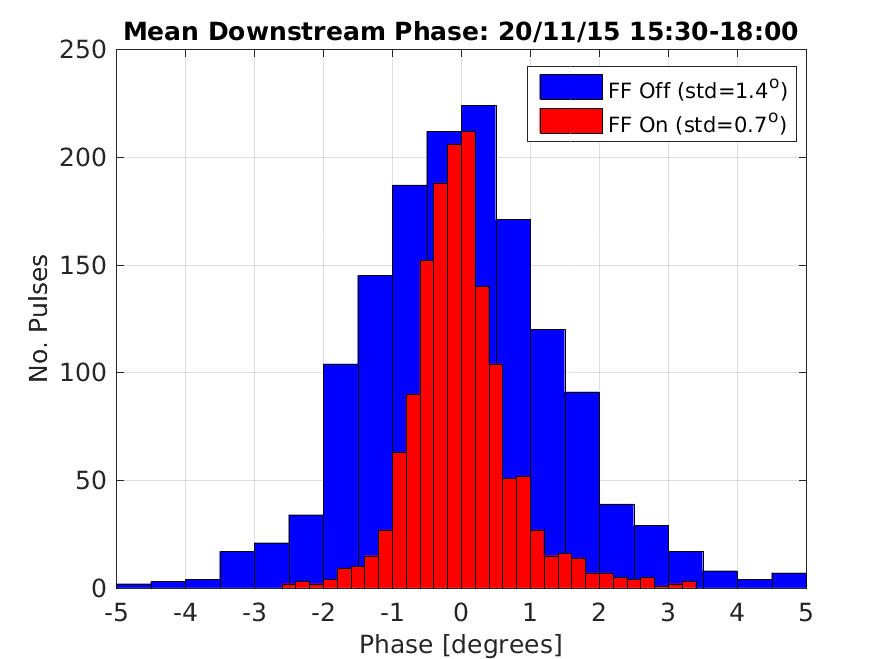
\includegraphics[width=0.45\textwidth]{Figures/feedforward/longFF_histDownstreamPhase}
  \caption{Histogram showing overall distribution of downstream phase with FF off and on.}
  \label{f:longFF_histDownstreamPhase}
\end{figure}

\begin{figure}
  \centering
  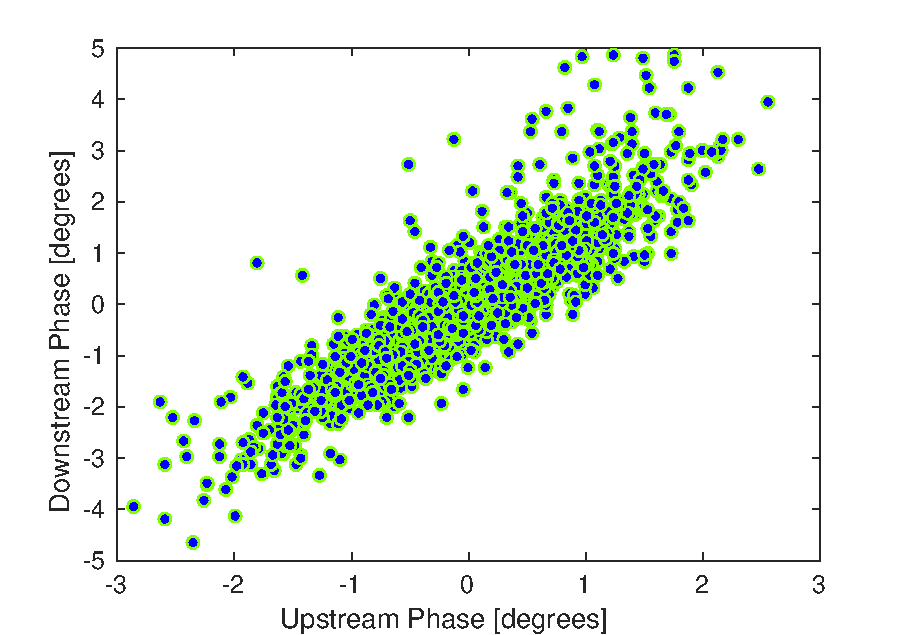
\includegraphics[width=0.45\textwidth]{Figures/feedforward/longFF_scatterFFOff}
  \caption{Downstream phase vs. upstream phase with FF off.}
  \label{f:longFF_scatterFFOff}
\end{figure}

\begin{figure}
  \centering
  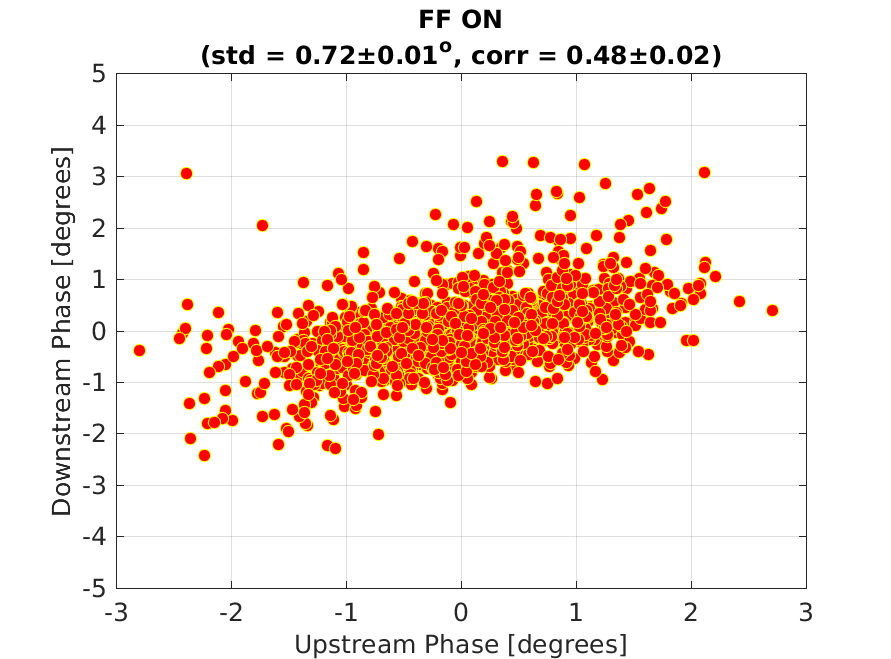
\includegraphics[width=0.45\textwidth]{Figures/feedforward/longFF_scatterFFOn}
  \caption{Downstream phase vs. upstream phase with FF on.}
  \label{f:longFF_scatterFFOn}
\end{figure}

\begin{figure}
  \centering
  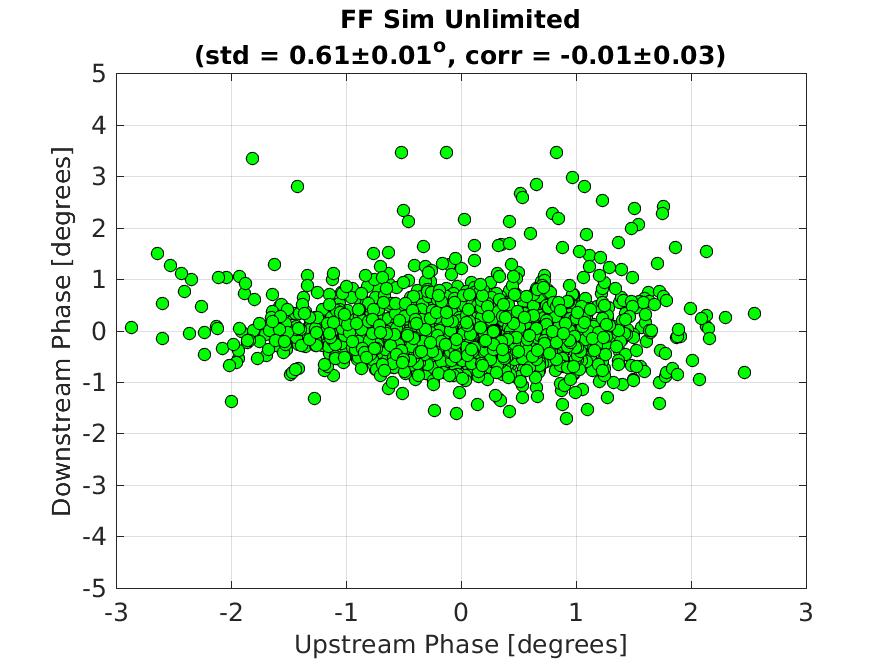
\includegraphics[width=0.45\textwidth]{Figures/feedforward/longFF_scatterFFSimOpt}
  \caption{Downstream phase vs. upstream phase with FF simulated at optimal gain.}
  \label{f:longFF_scatterFFSimOpt}
\end{figure}

\begin{figure}
  \centering
  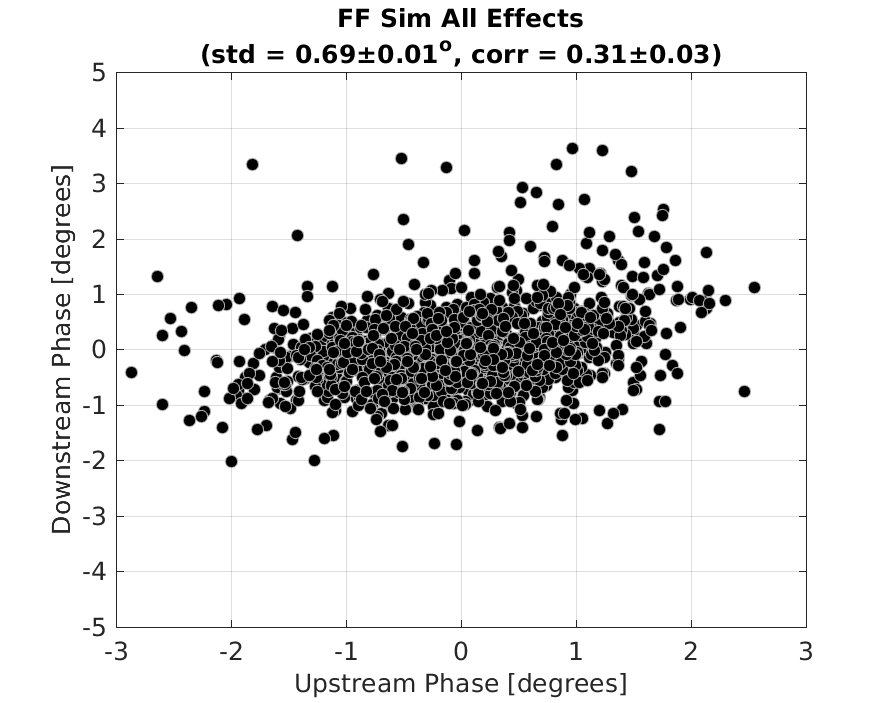
\includegraphics[width=0.45\textwidth]{Figures/feedforward/longFF_scatterFFSimReal}
  \caption{Downstream phase vs. upstream phase with FF simulated with actual gain used.}
  \label{f:longFF_scatterFFSimReal}
\end{figure}

\begin{table}
  \begin{center}
    \begin{tabular}{| c | c | c | c |}
	   \hline
       Correction Status & Upstream Jitter & Downstream Jitter & Correlation \\ \hline
       FF Off & \(0.88\pm0.02^\circ\) & \(1.40\pm0.03^\circ\) & \(0.89\pm0.01\) \\
	   FF On & \(0.86\pm0.02^\circ\) & \(0.72\pm0.01^\circ\) & \(0.48\pm0.02\) \\
	   FF Sim Opt Gain & \(0.88\pm0.02^\circ\) & \(0.61\pm0.01^\circ\) & \(-0.01\pm0.03\) \\
	   FF Sim Real Gain & \(0.88\pm0.02^\circ\) & \(0.68\pm0.01^\circ\) & \(0.35\pm0.02\) \\
	   FF Sim Offset & \(0.88\pm0.02^\circ\) & \(0.69\pm0.01^\circ\) & \(0.36\pm0.02\) \\
	   FF Sim 90\% Real Gain & \(0.88\pm0.02^\circ\) & \(0.72\pm0.01^\circ\) & \(0.46\pm0.02\) \\ \hline
    \end{tabular}
    \caption{Feedforward results using combined data from 20th November 2015.}
  	\label{t:LongFF}
  \end{center}
\end{table}



\newsection{pffNovelSetups}{Correction with Additional Jitter Source}

At CLIC the PFF system will be required to reduce the initial phase jitter by an order of magnitude, from 2 degrees to 0.2 degrees [REF]. With the initial phase jitter of typically 0.8 degrees at CTF3 it is not possible to demonstrate more than a factor 4 reduction in the jitter using the PFF prototype due to hardware limitations, more specifically due to the achieved phase monitor resolution of 0.14 degrees which limits the theoretical best possible correction to 0.2 degrees (Section \ref{s:resolution}). A secondary goal of the PFF prototype in addition to achieving the baseline goal of 0.2 degrees phase jitter is to demonstrate the factor 10 reduction in jitter relevant to CLIC. In order to do this additional sources of phase jitter must be added.

Clearly, the additional source must be prior to the upstream phase monitor in order to add an additional jitter component that is present in both the upstream and downstream monitors. The correlation between the resulting upstream and downstream phase must be  \(99.5\%\) in order for a factor 10 reduction in jitter to be possible (see Section \ref{ss:theoryJitter}). Two different methods to achieve this have been attempted --- firstly by varying the phases of all the klystrons in the injector and secondly by using the non-zero R56 stretching chicane (see Figure \ref{f:ctfLayout}) at the end of the CTF linac in order to intentionally add an energy component to the upstream phase (which propagates downstream).

\newsection{slowCorr}{Slow Correction}

As the PFF system has only a small range of \(\pm6^{o}\), a secondary ``slow phase feedback" or ``slow correction" has also been implemented at CTF3 to be able to remove larger drifts or static offsets in the downstream phase. In principle this slow correction can be used in conjunction with the PFF system to maximise its performance by keeping the mean uncorrected phase well-centred (zeroed) within its \(\pm6^{o}\) range so that the full power of the PFF amplifiers can be used to correct the fast pulse-to-pulse and intra-pulse phase jitter. If the beam phase were to drift away by \(15^{o}\), for example, the calculated PFF correction would saturate the amplifier across the full pulse length to give the maximal shift of \(6^{o}\). In this case the drift would be partially removed downstream but the PFF system would no longer have any effect on the phase jitter (as the output voltage to the kickers is constant in saturation rather than varying with the phase).

The design and results from the slow correction are discussed in this section. To date its main use has been to verify the ability to shift the beam phase in the TL2 chicane in early-2014 prior to the kicker amplifiers being available to commission the PFF system itself. The slow phase feedback has not yet been used in parallel with the PFF system apart from preliminary tests thus the results shown here are primarily a proof of principle. As PFF attempts have so far been predominantly taken in short datasets of up to a few hundred pulses any large drifts that arise can be manually removed between datasets, either by changing the correction setup (e.g. by changing the phase monitor phase shifters to re-zero the phase) or by re-establishing the previous beam conditions. The slow correction will however be an important tool for future attempts to demonstrate CLIC-level phase stability on time scales longer than a few minutes at CTF3.

\subsection{Implementation}
\label{ss:slowCorrMethod}

Ratio of corrector strengths for orbit closure.

\subsection{Results}
\label{ss:slowCorrResults}




